\documentclass{beamer}
\usepackage[cp1251]{inputenc}
%\usepackage[russian]{babel}
\usepackage{amsmath,mathrsfs,mathtext}
\usepackage{graphicx, epsfig}
\usetheme{Warsaw}%{Singapore}%{Warsaw}%{Warsaw}%{Darmstadt}
\usecolortheme{sidebartab}
\definecolor{beamer@blendedblue}{RGB}{15,120,80}
%----------------------------------------------------------------------------------------------------------
\title[\hbox to 56mm{Spherical convolutions  \hfill\insertframenumber\,/\,\inserttotalframenumber}]
{Quality prediction of proteins models with spherical convolutions on three-dimensional graphs}
\author[N.\,V.~Pavlichenko]{Nikita Pavlichenko}
\institute{Moscow Institute of Physics and Technology}
\date{\footnotesize{
\par\emph{Course:} My first scientific paper\par Group 793, 2020
\par\emph{Consultants:} I. Igashov, S. Grudinin
\date{qq}
}}
%----------------------------------------------------------------------------------------------------------
\begin{document}
%----------------------------------------------------------------------------------------------------------
\begin{frame}
%\thispagestyle{empty}
\titlepage
\end{frame}
%-----------------------------------------------------------------------------------------------------
\begin{frame}{Goal of research}
        \begin{itemize}
            \item Develop the new type of convolution operations on three-dimensional graphs that would be able to
            capture the 3D graph structure;
            \item Apply these operations to a node regression problem: prediction the quality of proteins model (Protein Quality Assessment).
        \end{itemize}
\end{frame}
%----------------------------------------------------------------------------------------------------------
\begin{frame}{Problem statement}
    \begin{itemize}
        \item Protein can be represented as a graph - a chain of amino acids
        \item Its properties are determined by its folding
        \item There are lots of folding models and it is expensive to find the right one for each protein experimentally
        \item Another way is to predict the quality of these models with machine learning algorithms - the regression problem on graphs.
        It also called Protein Quality Assessment problem
    \end{itemize}
\end{frame}

\begin{frame}{Problem statement}
    \includegraphics[width=1.0\textwidth]{img/protein_folding.png}
    \begin{itemize}
        \item Each protein model is described by a list of its amino residues
        \item Each residue has several features $x(v_i)$: its coordinates $(x, y, z)$ and one categorical feature - the one-hot encoded type of this residue.
        All rotated or biased models must be isomorphic.
        \item To construct a graph we build a Voronoi diagram on these amino residues. The cells of this diagram are nodes and
        if two cells have the same edge, we put an edge between corresponding nodes in the graph.
    \end{itemize}
\end{frame}

\begin{frame}{Problem statement}
    \begin{itemize}
        \item For each residue, we have a measure of the quality of its location - CAD score. It is already evaluated experimentally,
        so we will use it as a target for supervised learning.
        \item For each model $i$, we will predict the quality of each residue $j$. The common choice for loss
        function is MSE:
        $$\displaystyle{\sum_i^n \sum_j^{m_i}}(\hat{y}_{ij} - \text{CAD-score}_{ij})^2$$
    \end{itemize}
\end{frame}
%----------------------------------------------------------------------------------------------------------
\begin{frame}{Graph Convolutional Networks}
    For the last several years the most common approaches to Protein Quality Assessment include deep learning methods and Graph
    Colvolutional Networks in particular.
    \begin{block}{Idea}
        \begin{itemize}
            \item A very common method is Graph Convolutional Network
            \item $l$-th layer can be represented as $H^{(l)} = AH^{(l-1)}W^{(l)}$, where $A$ is the adjacency matrix, $W^{(l)}$ is weights matrix
        \end{itemize}
    \end{block}
    \begin{block}{Props and Cons}
        \begin{itemize}
            \item It was successfully applied for PQA before
            \item It does not capture a local protein structure
        \end{itemize}
    \end{block}
\end{frame}

\begin{frame}{Spherical convolutions}
        \begin{itemize}
            \item Amino acids are connected one by another so we can define a local coordinate system for every amino acid
            \item So, let's project it's neighbors onto a unit sphere.
            \item Consider a function of spherical coordinates. It can be expanded as a series of spherical harmonics.
             $$f(\phi, \psi) = \sum_{l = 0}^{\infty} \sum_{m=-l}^{m=l}f_l^m Y_l^m(\phi, \psi)$$
            \item Leave only a few coefficients and write it in a matrix view considering $\boldsymbol{W}_l^m$ a weight matrix
            $$f(\Omega) \approx f_W(\Omega) = \sum_{l=0}^{L}\sum_m \boldsymbol{W}_l^m Y_l^m(\Omega)$$
        \end{itemize}
\end{frame}
% , $A$ - adjcency matrix, $W^{(l)}$ - weights, $H^(l-1)$ - output of $l-1$-th layer
%----------------------------------------------------------------------------------------------------------
\begin{frame}{Spherical Convolutional Network}
        \begin{itemize}
            \item Introduce Spherical Convolution operation
            $$f_W \circ v_i = \sum_{v_j \in \mathcal{N}(v_i)} f_W(\Omega_i^j)x(v_i),$$
            where $\Omega_i^j$ denotes spherical coordiantes of the vertex $j$ in local coordinate system of the vertex $i$.
            \item Spherical convolution layer: $$\boldsymbol{X} \longrightarrow \boldsymbol{X}' = \sigma(f_W \circ \boldsymbol{X}) = \sigma\left(\sum_{l,m}Y_l^m(\boldsymbol{A}_\Omega)\boldsymbol{X}\boldsymbol{W}_l^m\right),$$
            $\boldsymbol{X} \in \mathbb{R}^{n\times d}$ - input features, $\boldsymbol{X}' \in \mathbb{R}^{n\times d'}$ - output features, $\sigma$ - non-linearity e.g. ELU.
            \item Learn $\boldsymbol{W}_l^m$ matrices using Adam optimizer
        \end{itemize}
   %\includegraphics[width=0.7\textwidth]{fig/ErrorFunction}
\end{frame}

\begin{frame}{Computational experiment}
    To compare the proposed approach we have trained both GCN and SCN networks on CASP data and compared the quality metrics.
    \begin{block}{Dataset}
        \begin{itemize}
            \item We use CASP competition data - more than 100k protein models made by participants and scored experimentally to get the CAD-score. CASP8-11 (80k models) as a training sample and CASP12 (5k models) as a testing sample.
            \item Spherical harmonics are precalculated: we use an order of 5 and it takes 60GB of HDD
        \end{itemize}
    \end{block}
    
   %\includegraphics[width=0.7\textwidth]{fig/ErrorFunction}
\end{frame}
%----------------------------------------------------------------------------------------------------------
\begin{frame}{Computational experiment}
    \begin{block}{GCN baseline}
        \begin{itemize}
            \item 8 GCN layers with 4 linear layers at the beginning as an encoder and 5 linear layers at the end is the best setup for GCN
            \item Learn on CPU since the loading from HDD is a bottleneck
        \end{itemize}
    \end{block}
    \begin{block}{Algorithm}
        \begin{itemize}
            \item Optimal architecture is 5 spherical convolution layers
            \item All code is written in PyTorch
            \item Learn on GPU in 4 parallel subprocesses
        \end{itemize}
    \end{block}
\end{frame}
\begin{frame}{Computational experiment}
    \begin{block}{Results}
        \begin{itemize}
            \item The common choice for a quality metric is the Pearson correlation between ground truth and predictions
            \item The best achieved result for GCN is $0.57$ comparing with $0.787$ with spherical convolutions
        \end{itemize}
    \end{block}
    \begin{table}[H]
        \centering
        \begin{tabular}{l|l|l|l|l}
            \hline
                   & $\rho$ &  $r$     &   rank       & z-score \\ \hline
        ProQ3D     & 0.801  &  0.750   &   11.961     & 1.670       \\
        VoroMQA    & 0.803  &  0.766   &   17.171     & 1.410       \\  
        SBROD      & 0.685  &  0.762   &   23.579     & 1.282       \\
        Ornate     & 0.828  &  0.781   &   10.776     & 1.780       \\
        \textbf{GCN}        & 0.570  &  0.510   &   31.667     & 0.979       \\
        \textbf{SCN}        & 0.787  &  0.720   &   18.462     & 1.411       
    \end{tabular}
    \caption{Comparsion of Pearson, Spearman correlation coefficients and z-score and rank of the state-of-the-art algorithms,
        our GCN baseline and Spherical Convolutional Network on CASP12 dataset.
        }
    \label{Tab:1}
    \end{table}
    
   %\includegraphics[width=0.7\textwidth]{fig/ErrorFunction}
\end{frame}
\begin{frame}{Computational experiment}
    Learning curves of two algorithms show that SCN achieves better results with fewer iterations
    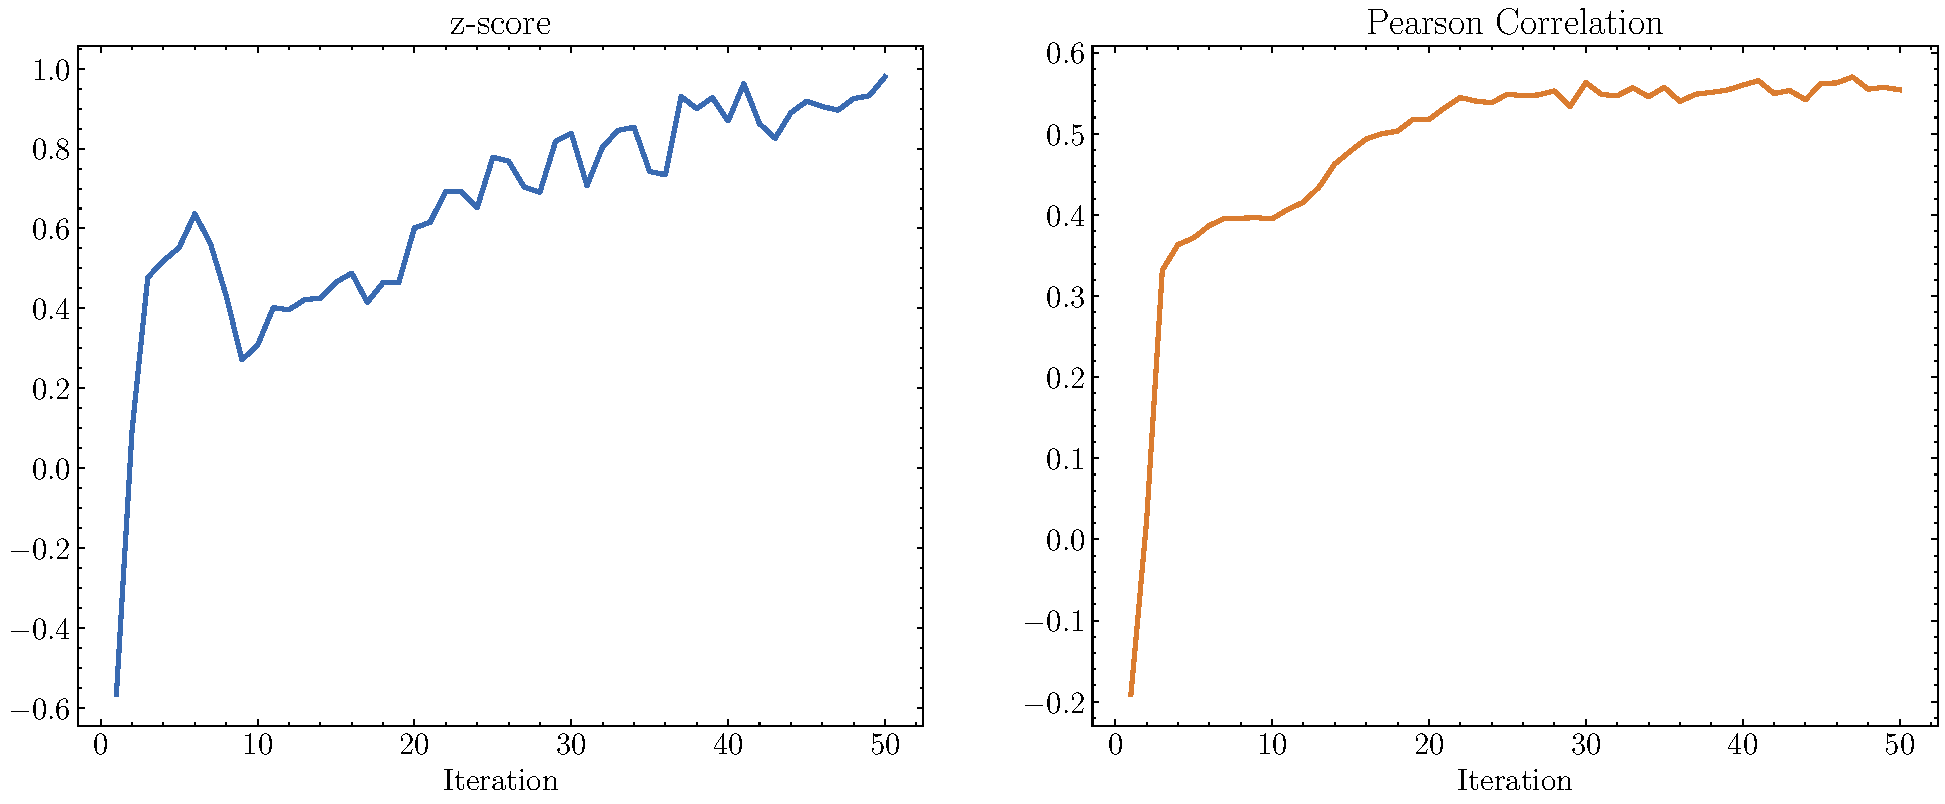
\includegraphics[width=1.0\textwidth]{img/z_score_casp12.pdf}
    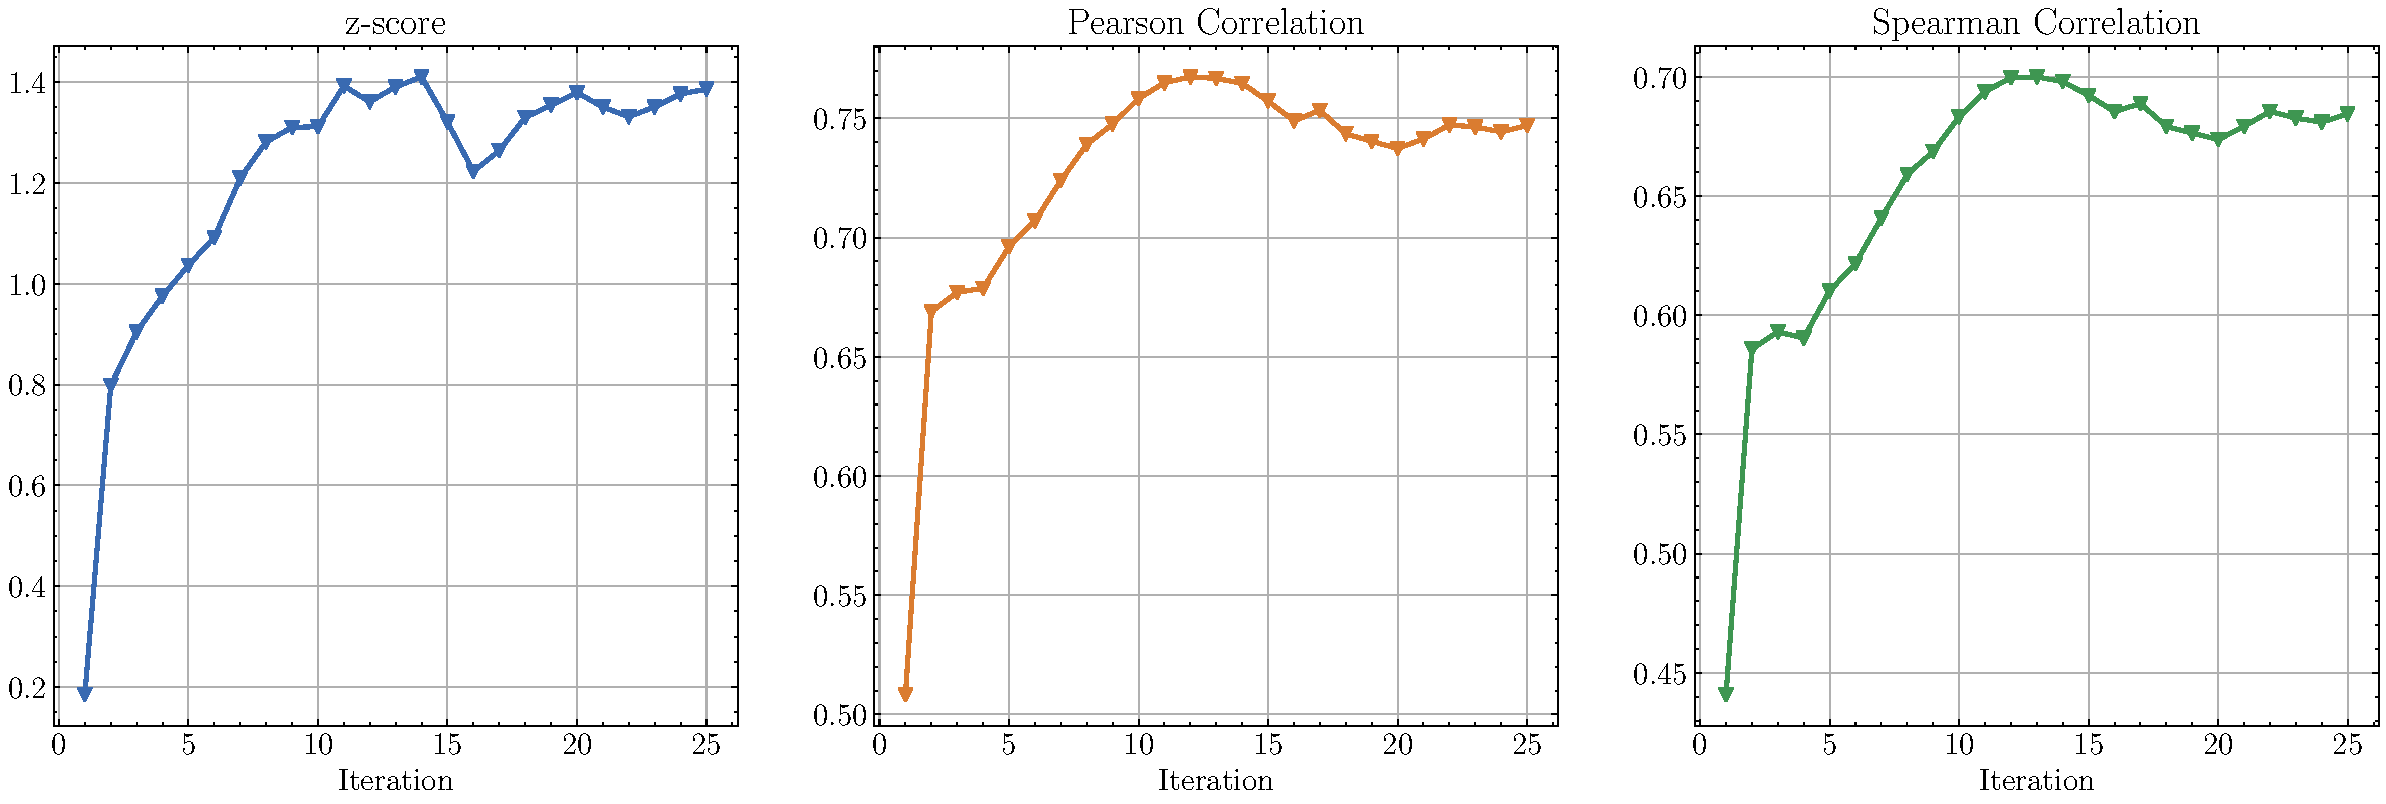
\includegraphics[width=1.0\textwidth]{img/z_score_casp12_sh.pdf}
   %\includegraphics[width=0.7\textwidth]{fig/ErrorFunction}
\end{frame}
\begin{frame}{Conclusion}
        \begin{itemize}
            \item SCN has shown significantly better performance comparing with GCN. This result can be even compared with
            the state-of-the-art approaches that include genetic and biology features that represent protein evolution
            \item It has proved the hypothesis that the most significant property of the protein is its geometric structure
        \end{itemize}
\end{frame}
\begin{frame}{Further research}
    \begin{itemize}
        \item Combine SCN approach with features engineered for GraphQA, VoroCNN, and other state-of-the-art algorithms
        \item Try spherical convolution layers in other graph neural network structures such as variational autoencoders
    \end{itemize}
\end{frame}
%----------------------------------------------------------------------------------------------------------
\end{document} 
